\documentclass[sigconf]{acmart}
\usepackage{booktabs} % For formal tables

% Copyright
%\setcopyright{none}
%\setcopyright{acmcopyright}
%\setcopyright{acmlicensed}
\setcopyright{rightsretained}
%\setcopyright{usgov}
%\setcopyright{usgovmixed}
%\setcopyright{cagov}
%\setcopyright{cagovmixed}

%Conference
\acmConference[KDD'2017]{ACM Transactions on Knowledge Discovery from Data}{August 2017}{Halifax, Nova Scotia - Canada} 
\acmYear{1997}
\copyrightyear{2016}

\usepackage{pgfplotstable}
\usepackage{caption}
\usepackage{subcaption}

\usepackage[noend]{algpseudocode}

\usepackage{float}
\usepackage{amsmath}

\usepackage[ruled]{algorithm2e} % For algorithms
\renewcommand{\algorithmcfname}{ALGORITHM}
\SetAlFnt{\small}
\SetAlCapFnt{\small}
\SetAlCapNameFnt{\small}
\SetAlCapHSkip{0pt}
\IncMargin{-\parindent}



%\acmBadgeR[http://ctuning.org/ae/ppopp2016.html]{ae-logo}
%\acmBadgeL[http://ctuning.org/ae/ppopp2016.html]{ae-logo}


% DOI

% Paper history
%\received{February 2017}
%\received{March 2017}
%\received[accepted]{June 2017}


% Document starts
\begin{document}
% Title portion
\title{LDA Model Monitoring in Distributed Streaming System} 
\author{Ran Bernstein}
\affiliation{%
  \institution{Technion -- Israel Institute of Technology}
  \department{Computer Science}
  \city{Haifa}
  \postcode{32000}
  \country{Israel}
  }
  \email{bernstein.ran@Gmail.com}
  
\author{Margarita Osadchy}
\affiliation{%
  \institution{University of Haifa}
  \department{Computer Science}
  \city{Haifa}
  \postcode{31905}
  \country{Israel}
}
\email{rita@cs.haifa.ac.il}

\author{Daniel Keren}
\affiliation{%
  \institution{University of Haifa}
  \department{Computer Science}
  \city{Haifa}
  \postcode{31905}
  \country{Israel}
}
\email{dkeren@cs.haifa.ac.il}

\author{Assaf Schuster}
\affiliation{%
  \institution{Technion -- Israel Institute of Technology}
  \department{Computer Science}
  \city{Haifa}
  \postcode{32000}
  \country{Israel}
}
\email{assaf@cs.technion.ac.il}

\begin{abstract}
Real systems for mining data streams should be able to detect changes that affect the accuracy of the dynamic model describing the temporal data. A distributed setting poses one of the main challenges in this type of change detection. In a distributed setting, model training requires centralizing the data from all nodes (hereafter, synchronization), which is very costly in terms of communication. In order to minimize communication, a monitoring algorithm should be executed \emph{locally} at each node,
while preserving the validity of the global model (that is, the model that will be computed if a synchronization takes place). To achieve this goal, we propose the first communication-efficient algorithm for monitoring a classification model over distributed, dynamic data streams. The classifier we monitor is the Linear Discriminant Analysis (LDA), a popular method for classification and dimensionality reduction in many fields. Please note that the emphasis of this work is \emph{not} on solving the distributed optimization problem
that corresponds to finding a classifier over the distributed data; instead, we continuously
monitor the current classifier to check that it still fits the data.

In addition to the theoretical guarantee of the proposed monitoring algorithm, we demonstrate how it reduce communication volume by up to two orders of magnitude (compared to synchronization in every round) on three real data sets from different worlds of content, as well as its advantage over the
popular periodic sampling paradigm. Moreover, our approach monitors the \emph{classification model itself} as opposed to its misclassifications, which makes it possible to detect the change before misclassification occurs.
\end{abstract}


%
% The code below should be generated by the tool at
% http://dl.acm.org/ccs.cfm
% Please copy and paste the code instead of the example below. 
%
\begin{CCSXML}
<ccs2012>
<concept>
<concept_id>10002951.10003227.10003351.10003446</concept_id>
<concept_desc>Information systems~Data stream mining</concept_desc>
<concept_significance>500</concept_significance>
</concept>
<concept>
<concept_id>10010147.10010257.10010293.10010307</concept_id>
<concept_desc>Computing methodologies~Learning linear models</concept_desc>
<concept_significance>300</concept_significance>
</concept>
<concept>
<concept_id>10010147.10010919.10010172</concept_id>
<concept_desc>Computing methodologies~Distributed algorithms</concept_desc>
<concept_significance>300</concept_significance>
</concept>
</ccs2012>
\end{CCSXML}

\ccsdesc[500]{Information systems~Data stream mining}
\ccsdesc[300]{Computing methodologies~Learning linear models}
\ccsdesc[300]{Computing methodologies~Distributed algorithms}


%
% End generated code
%


\keywords{Distributed Monitoring, Linear Discriminant Analysis}


\maketitle

\section{Introduction}

We address the problem of classifying streaming data which
is \textit{distributed} over a large number of nodes. The streaming data distribution is not stationary, and can change over time. Popular examples of real-life problems that involve this kind of change are user preference prediction and fraud detection. In the former, the choices of the user can change over time; in the latter, the fraudulent transactions are constantly changed to avoid detection. In both cases, the change can render the classifier invalid.
In such a setting --- where the model must be updated to stay valid and communication is costly --- the question is \textit{when} to recompute the model. The naive solution for this problem is recomputing the model periodically. The problem with this solution is that it involves needless work if the model changes infrequently, yet may introduce unacceptable errors between scheduled updates. 
In contrast to periodical computation, we focus on \textit{monitoring} the quality of a given model, and recomputing it only when necessary. 
\par We focus on linear binary classifiers, using LDA \cite{fisher1936use} as the classifier. This choice is motivated by the popularity of linear classifiers in real applications, and their usage as a platform for more complex classifiers, such as ensemble model in the work of ~\cite{Deva, eSVM}, neural networks in the work of ~\cite{osadchy2015k}, 
and even deep architectures in the work of \cite{ROSS}. Our method is distinct from the previous work in the following two important aspects:

\noindent \textbf{Model-Based Monitoring:} 
In contrast to most previous work on monitoring a classifier (that utilizes misclassification rate to draw conclusions about the change in the distribution 
\cite{baena2006early, gama2004learning, nishida2007detecting}), we propose to monitor the change in the \textit{model itself}.
Monitoring the model, and not just its misclassifications, has an important benefit: the need for synchronization can be detected before misclassifications occur. 

\noindent \textbf{Distributed Setting:} 
We note here that the problem we tackle is quite different from distributed
{\em computation} of a classifier \cite{macua2011distributed}, and also
from incrementally updating it\cite{pang2005incremental}. Here,
we assume that the classifier was already constructed, but that new data
keeps flowing into a set of distributed nodes. For this scenario, we propose a
{\em tracking} mechanism, which does not keep updating the classifier, but
quickly checks whether its initial value had changed by more than a
pre-defined threshold. This stage is done while maintaining a small
communication overhead between the nodes. Only if the threshold
is violated, a communication protocol is activated. While local alert
mechanism for detecting concept drift in distributed environments
were studied before (~\cite{AngGZPH13}), our approach is, to the best of our knowledge, the only one that provides a provable guarantees of correctness. 

\section{Related Work on Distributed Monitoring}
Monitoring dynamic data streams is a broad topic which was addressed in different research communities. We focus on detecting changes in the stream that render the current data model invalid. 
In distributed settings, this problem is notably more difficult than in the centralized case; it is typically referred to as \textit{distributed monitoring}, and it is concerned with designing local tests for monitoring a function that is defined globally over all the nodes in the system.
Our approach to this problem is to define a constraint over the local data (at each node) that guarantees the validity of the global model. If local data (in one or more nodes) does not meet the local condition, it leads to synchronization. The synchronization process suffers from a high communication cost, and the goal of the distributed monitoring protocol is thus to minimize the number of synchronizations. Most work on distributed monitoring has been concerned with simple functions, such as linear functions in the work of ~\cite{keralapura2006communication} and ~\cite{kashyap2008efficient}, or monotonic functions in the work of \cite{michel2005klee}.
For non-linear functions, examples include work on monitoring the value
of a single-variable polynomial as in  ~\cite{shah2008handling},
and eigenvalue perturbation as in the work of ~\cite{huang2007communication}.
While the previous work handled specific families of functions, we chose to use the 
\textit{geometric approach} for monitoring \textit{arbitrary} functions over distributed streams, as was proposed, and later extended and generalized in \cite{sharfman2007geometric, keren2014geometric, keren2012shape,gabel2015monitoring}. 
%A recently introduced work by 
%~\cite{gabel2015monitoring} on monitoring Least % 
%Square Regression (LSR) using geometric monitoring is the closest in %spirit to this work, but our problem is more complex, as
%computing the LSR model requires only solving a convex optimization %problem, while
%computing the LDA classifier cannot be cast in this way.
%
\section{Problem Definition}
We first describe the Linear Discriminant Analysis (LDA) algorithm and then define the monitoring problem. 

\subsection{Linear Discriminant Analysis}%\\ \par
LDA seeks a linear combination of features that characterize or separate two or more classes of samples.
The resulting combination may be used as a linear classifier, or for dimensionality reduction before subsequent classification.

The classification problem is solved by first assuming that the conditional probability
density functions $Pr(\vec x|y=p)$ and $Pr(\vec x|y=q)$ are both normally distributed, with
mean and covariance  $(p, B_p)$ and
$(q, B_q)$, for two target classes $P$ and $Q$ respectively.\\
${(x_1,y_1),\ldots,(x_n,y_n)}$ are i.i.d. samples, $x_i \in \mathbb{R}^d$
and $y_i \in \{0,1\}$.

We seek a linear projection defined by an inner product with a vector $w \in \mathbb{R}^d $,
that maximizes the separation between the classes, where the separation is
defined to be the ratio of the variance between the classes to the variance
within the classes:
\begin{equation}
\frac{\sigma^2_{between}}{\sigma^2_{within}} = \frac{(w^T (p -
q))^2}{w^T(B_p+B_q)w}.
\end{equation}
Solving the maximization problem yields that the decision criterion is a threshold on the
dot product
\begin{equation*} \label{eq:decision}
w \cdot x > c
\end{equation*}
where
\begin{equation} \label{eq:w}
w \propto (B_p+B_q)^{-1}(p - q)
\end{equation}
\begin{equation} \label{eq:c}
c = \frac{1}{2}(T-{p}^T S_p^{-1} {p}+{q}^T S_q^{-1} {q}).
\end{equation}
In this work we monitor $w$, and will refer to it as the classification \textit{model}.

\subsection{Monitoring Problem}
\label{sub:problem}
We denote the number of nodes by $k$ and the number of samples in a node by $W$.
Our model assumes discrete time (hereafter, rounds). Every node receives a new sample
in every round. We use the \textit{sliding window} model; every node keeps two sliding windows (one for each class) of length $W/2$. As a node receives a new observation, it replaces the oldest one from its class.
$x^i_j$ and $y^i_j$ are the $j$'th sample and label in the $i$'th node
and $x_{old}^i(p)$, $x_{old}^i(q)$ are the oldest samples from each class in
the sliding window of the $i$'th node.
As data evolves, it is possible that the previously computed model
no longer matches the current true model. Let $w_0$ be the last computed model, i.e. computed at the most recent synchronization, and let $w$ be the \textit{true} LDA model (the hypothetical model that a present synchronization would yield). So,
we must bound the deviation of $w_0$ from $w$.
For the classification purpose, the most important property of a linear classifier is its direction. Therefore, we monitor the change in this direction: given a threshold $T$, our goal is to raise an alert if
\begin{equation} \label{eq:coneCritiria}
\frac{<w,w_0>}{\parallel w \parallel \parallel w_0 \parallel}  < T.
\end{equation}
i.e. if the angle between $w_0$ and $w$ is above a certain threshold (the inner product between unit vectors is the cosine of the angle between them). Note that this
defines a cone in Euclidean space -- that is, $w$ is valid as long as it is
contained in a cone whose apex is $w_0$; the cone's opening angle determines
the amount of "slack" by which $w$ is allowed to deviate from $w$.

%Due to the complexity of Eq. \ref{eq:coneCritiria},
%we will monitor a simpler problem whose solution also satisfies
Next, we replace the cone containment condition to a (solid) sphere containment condition, i.e., 
%Eq. \ref{eq:coneCritiria}: the maximal volume sphere of which $w_0$ is its center
%that resides completely inside the cone from Eq. ~\ref{eq:coneCritiria}.
%This sphere is defined by
\begin{equation} \label{eq:critiria}
||w-w_0||   \leq  R_0,
\end{equation}
where $R_0 := ||w_0|| \sqrt{1-T^2}$ is the radius of the maximal volume sphere with center $w_0$, and
which resides inside the cone from condition \ref{eq:coneCritiria}. A probabilistic justification for
this replacement\footnote{It is possible to compare the probabilities of a random vector, from a
distribution centered at $w_0$, to fall in the sphere or in the cone.} is too long to 
include here; we provide an example in the experiments section 
(Fig. \ref{CosineVsEuclideanPowerSupply}).

%In other words, we replaced containment by distance from the boundary.
%Empirical evaluation showed that the values of
%$1-\frac{<w,w_0>}{||w||||w_0||}$ and $||w-w_0||$ are
%highly  correlated, thus in practice, Eq. \ref{eq:coneCritiria}
%can be replaced by Eq.\ref{eq:critiria}.


\section{Monitoring Distributed LDA with Safe Zones}
Locally monitoring distributed LDA models poses a non-trivial difficulty, since the global model cannot be inferred from the local models at each node. Even when all current local models $w_i$ are identical to the precomputed global model $w_0$, the current global model $w$ may be very different from  $w_0$: consider the example in Figure \ref{NegativeExample} with $k = 2$ nodes and dimension $d =2$. The deviation
in the orientation of the global model (blue lines) over time is very large ($45^{\circ}$) even though the orientations of the local models (green and red lines) are identical to their
initial values.

\begin{figure}[H]
\centering
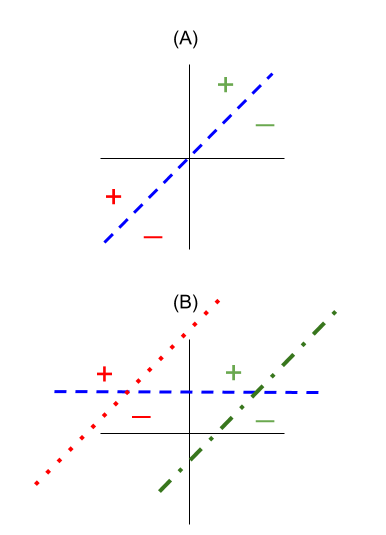
\includegraphics[width=50mm, height=6cm]{graphics/NegativeExample.png}
\caption{Example of incorrect monitoring by observing only the local LDA classifiers. The
initial state of the data is depicted in (A) and the state at a later point
in time
in (B), where the positive samples are concentrated around the "+" signs and
the negative ones around the "-" signs; green and red represent the two classes.
In configuration (B), every node  calculates the same orientation
for the LDA classifier as it was in (A) -- i.e., the node's \emph{local view} is
stationary. However, the orientation of the global data classifier (blue line) had very
significantly changed from (A) to (B).}
\label{NegativeExample}
\end{figure}


\par To overcome this difficulty, we impose constraints on the local data at the nodes, rather than on the 
local classifier. Specifically, we assign certain subsets, referred to as \textit{safe zones}, to each node,
such that as long as local data remains inside the safe zones, it is guaranteed that the function of the global average ---  i.e. the Euclidean distance between the true global model to the one that was computed in the last synchronization (hereafter, \emph{model drift}) --- does not cross the threshold.
In other words, we want to impose conditions on the local
data at each node so that as long as they hold, $||w-w_0|| \leq R_0$, i.e., the global model is valid.

Nodes communicate only when the local data exits the
safe zone, i.e.  a safe zone \textit{violation} (hereafter, just
violation) occurs. Once that happens, violations can be resolved,
for example by synchronization.


\subsection{Notation}
\noindent
We recall that $P$ and $Q$ are the classes in the binary classification problem.
 $(p,q)$ and $(p^i,q^i)$  are the global and local means of classes $P$ and $Q$.
$S$ and $S^i$  are the global and local normalized scatter matrices of the feature space:
\begin{equation*}
S^i := \frac{1}{W}\sum_{j=1}^{W}x^i_j(x^i_j)^T
\end{equation*}
\begin{equation*}
S := \frac{1}{Wk}
\sum_{i=1}^k\sum_{j=1}^Wx^i_j(x^i_j)^T=\frac{1}{k}\sum_{i=1}^kS^i.
\end{equation*}
\\Similarly, $u$ and $u^i$ are the differences between the means of the classes, i.e., $u:=p - q$ and $u^i:=p^i - q^i$.
\\ $B$ is the global covariance matrix, which is the sum of the covariance matrices of the two classes, i.e., $B:=B_p+Bq$.
It can be shown that $B=S - pp^T - qq^T$.
%\\B^i:=S^i - p^i(p^i)^T - q^i(q^i)^T$
\\Let $w$ be our current true model. Then, following Eq.~\ref{eq:w}, we can write:
%\\$w(S,\mu_p,\mu_q) := (S - \mu_p\mu_p^T - \mu_q\mu_q^T)^{-1}(\mu_p - \mu_q)$
\begin{equation}
w:=(S - pp^T - qq^T)^{-1}(p-q)=B^{-1}u.
\end{equation}
%In the following the subscript $0$ will denote the state at the time
%of last synchronization.
Let $w_0$ be the existing model, previously computed from $(S_0, p_0, q_0)$
or from $(B_0,u_0)$ at the time of synchronization.
Then,
\begin{equation}
w_0:=(S_0 - p_0p_0^T - q_0q_0^T)^{-1}(p_0-q_0)=B_0^{-1}u_0.
\end{equation}

If $S_0^i$, $p_0^i$ and $q_0^i$ are the local normalized scatter and averages
of the samples in a node at the time of last synchronization, we define the \textit{local drifts} to be:
\begin{alignat*}{1}
& \Delta_s^i:= S^i - S_0^i
\\ & \delta_p^i:= p^i - p_0^i
\\ & \delta_q^i:= q^i - q_0^i.
\end{alignat*}
We define $\Delta_s, \delta_p$, and $\delta_q$ --- the \textit{global drift} vectors of $S, p$, and $q$ -- to be:
\begin{alignat*}{1}
& \Delta_s:= S - S_0 \\
& \delta_p:= p - p_0 \\
& \delta_q := q - q_0.
\end{alignat*}

\begin{remark} \label{average}
It is easy to see that every global drift vector is the average of the local drift vectors:
\begin{alignat*}{1}
& \Delta_s = \frac{1}{k} \sum \Delta_s^i, \\
& \delta_p = \frac{1}{k} \sum \delta_p^i, \\
& \delta_q = \frac{1}{k} \sum \delta_q^i.
\end{alignat*}

\end{remark}

\subsection{Constructing Safe Zones}
Each node monitors its own drift vector: as long as the current values
at the nodes, $(S^i,p^i,q^i)$, satisfy a certain condition w.r.t their
values 
at synchronization time $(S^i_0,p^i_0,q^i_0)$, $w_0$ is guaranteed to be close to $w$.
This condition is defined as containment in a certain \textit{convex} safe zone. 
Formally, we shall define a convex set $\mathcal{C}$ such that:
\begin{equation} \label{convex}
(\Delta_s, \delta_p, \delta_q) \in \mathcal{C} \Rightarrow \parallel w-w_0
\parallel \ \leq R_0.
\end{equation}
\begin{lemma} \label{averages}
Let $\mathcal{C}$ be a convex set that satisfies Eq. \ref{convex}.
If \\
$(\Delta_s^i, \delta_p^i, \delta_q^i) \in \mathcal{C}$ for all i, then
\begin{equation*}
||w-w_0|| \leq R_0.
\end{equation*}
\end{lemma}
\begin{proof}
We express $S, p$ and $q$ as their values at synchronization with the addition of the average of the local drift vectors:
\begin{equation}
\begin{split}
\\(S,p,q) & = \frac{1}{k} \sum_i (S^i,p^i,q^j) \\
 & = (S_0,p_0,q_0) + \frac{1}{k} \sum_i (\Delta_s^i,\delta^i_p,\delta_q^i). \\
\end{split}
\end{equation}
From $\mathcal{C}$'s convexity  we obtain
\begin{equation}
\begin{split}
\forall i (\Delta_s^i,\delta^i_p,\delta_q^i) \in \mathcal{C} & \Rightarrow
\frac{1}{k} \sum_i (\Delta_s^i,\delta^i_p,\delta_q^i) \in \mathcal{C} \\
& \Rightarrow (\Delta_s,\delta_p,\delta_q) \in \mathcal{C}.
\end{split}
\end{equation}
Finally, from the definition of $\mathcal{C}$ we obtain:
\begin{equation}
(\Delta_s,\delta_p,\delta_q) \in \mathcal{C} \Rightarrow \parallel w-w_0
\parallel \ \leq R_0,
\end{equation}
\end{proof}
We note the following:
\begin{itemize}
    \item The convexity of \mathcal{C} is crucial in order to allow "going from
    local to global", i.e. inferring a global condition on the global $w$ from
    local conditions which can be checked individually at each node.
\item The set $\mathcal{C}$ is defined not in the space of vectors $w$, but in
Euclidean space of dimension $n^2+2n$, where $n$ is the dimension of $w$.
\end{itemize}

\subsection{Constructing the Safe Zones}
Denote the change in the global covariance matrix
\begin{alignat*}{2}
\Delta & := && B-B_0 \\
& = && (S_0+\Delta_S - (p_0+\delta_p)(p_0+\delta_p)^T \\
& && - (q_0+\delta_q)(q_0+\delta_q)^T) \\
& && - (S_0 - p_0p_0^T - q_0q_0^T) \\
& = && - \delta_p\delta_p^T - \delta_q\delta_q^T \\
& && + \Delta_S - p_0\delta_p^T \\
& && - \delta_pp_0^T - q_0\delta_q^T - \delta_qq_0^T.
\end{alignat*}
Next, separate $\Delta$ into its quadratic part,
\begin{equation*}
M:= - \delta_p\delta_p^T - \delta_q\delta_q^T
\end{equation*}
\begin{equation*}
M^i = - \delta_p^i(\delta_p^i)^T - \delta_q^i(\delta_q^i)^T
\end{equation*}
and its linear part,
\begin{equation*}
L:= \Delta_S - p_0\delta_p^T - \delta_pp_0^T - q_0\delta_q^T - \delta_qq_0^T
\end{equation*}
\begin{equation*}
\\ L^i := \Delta_S^i - p_0^i(\delta_p^i)^T - \delta_p^i(p_0^i)^T -
q_0^i(\delta_q^i)^T - \delta_q^i(q_0^i)^T,
\end{equation*}
hence
\begin{equation*}
\Delta= L+ M, 
\end{equation*}
\begin{equation*}
\Delta^i:= L^i+ M^i.
\end{equation*}
We denote the change of the distance between the means as
\begin{equation*}
\delta:= u-u_0 = \delta_p - \delta_q, 
\end{equation*}
\begin{equation*}
\delta^i:=\delta_p^i - \delta_q^i.
\end{equation*}
Now we can now define $\mathcal{C}$ as follows:
\begin{lemma} \label{lemma:convexBound}
Let $\mathcal{C}$ be the set of triplets $(\Delta_s^i, \delta_p^i, \delta_q^i)$
 that satisfy the inequality:
 \begin{equation} \label{eq:convexBound}
||B_0^{-1}\delta^i|| + \left(||w_0||+R_0\right)\left(||B_0^{-1}L^i}|| + 
||B_0^{-1}M^i}||\right) \leq  R_0
\end{equation}
where $||\cdot||$ stands for the operator norm in case the
argument is a matrix, and the Euclidean norm if the argument is a vector.

\\Then, if $||{B_0^{-1}\Delta^i}|| < 1$ for every $i$, 
Eq. \ref{eq:critiria} holds; further, $\mathcal{C}$ is convex.
\end{lemma}
The proof of Lemma \ref{lemma:convexBound} cannot be included due to space limitations.

\section{Distributed LDA Monitoring Algorithm}
We now present two frameworks for LDA model monitoring that use
the bound in Eq. \ref{eq:convexBound}. 
In both frameworks, 
we assign a \textit{coordinator}, whose task is to monitor the violation alerts from the nodes and aggregate the data from all the nodes when a violation occurs. The coordinator recomputes the model after data aggregation, and sends the updated covariance matrix 
and class averages to the nodes.
In both frameworks, every node runs the same
update algorithm as detailed in Alg. \ref{NodeUpdate}.
The frameworks differ in their synchronization policy; 
the first, Distributed LDA Monitoring (DLDA), will synchronize in a round
in which at least one node  reported a violation (condition \ref{eq:convexBound} in the node is not satisfied as detailed in Alg.~\ref{DLDA}).
The second, Probabilistic Distributed LDA Monitoring (PDLDA), will synchronize in a round in which the number of nodes with a violation is above a certain
threshold.
The derivation of this threshold is presented in Section \ref{sec:PDLDA}.


\begin{algorithm}
\SetAlgoNoLine
\KwIn{$i$ is the index of the node, $(x,y)$ is a new sample.}
%\Procedure{Update}{}
\If {$y$ is class P}
{ $p^i = p^i + x - x_{old}^i(p)$ \;
 $S^i = S^i +xx^T - x_{old}^i(p)(x_{old}^i(p))^T$}
\Else
{$q^i = q^i + x -x_{old}^i(q)$ \;
 $S^i = S^i +xx^T - x_{old}^i(q)(x_{old}^i(q))^T$ \;
$(\Delta_s^i,\delta^i_p,\delta_q^i) = (S^i-S^i_0,p^i-p^i_0,q^i-q^i_0)$ }
%\If{The bound in \ref{eq:convexBound} is not satisfied}

\If { $||B_0^{-1}\delta^i||+ (||w_0||+R_0)(||B_0^{-1}L^i||+||B_0^{-1}M^i||) >R_0$}
{Report violation to coordinator \;
Receive new global $B_0^{-1}$, $w_0$ \;
$(S_0^i,p_0^i,q_0^i) = (S^i,p^i,q^i)$ }

\caption{Node Update}

\label{NodeUpdate}
\end{algorithm}


\begin{algorithm}
\SetAlgoNoLine
\caption{Coordinator synchronization algorithm.}\label{DLDA}
\If {One of the nodes has reported for violation} 
{
Collect data from the nodes \;
Receive from every node $i$ the triplet $(S^i,p^i,q^i)$ \;
Compute updated $w_0$ and $B_0^{-1}$ and distribute.}
\end{algorithm}
%
\subsection{Probabilistic Distributed LDA Monitoring}\label{sec:PDLDA}
%





\begin{figure*}
\centering
\begin{minipage}{.7\textwidth}
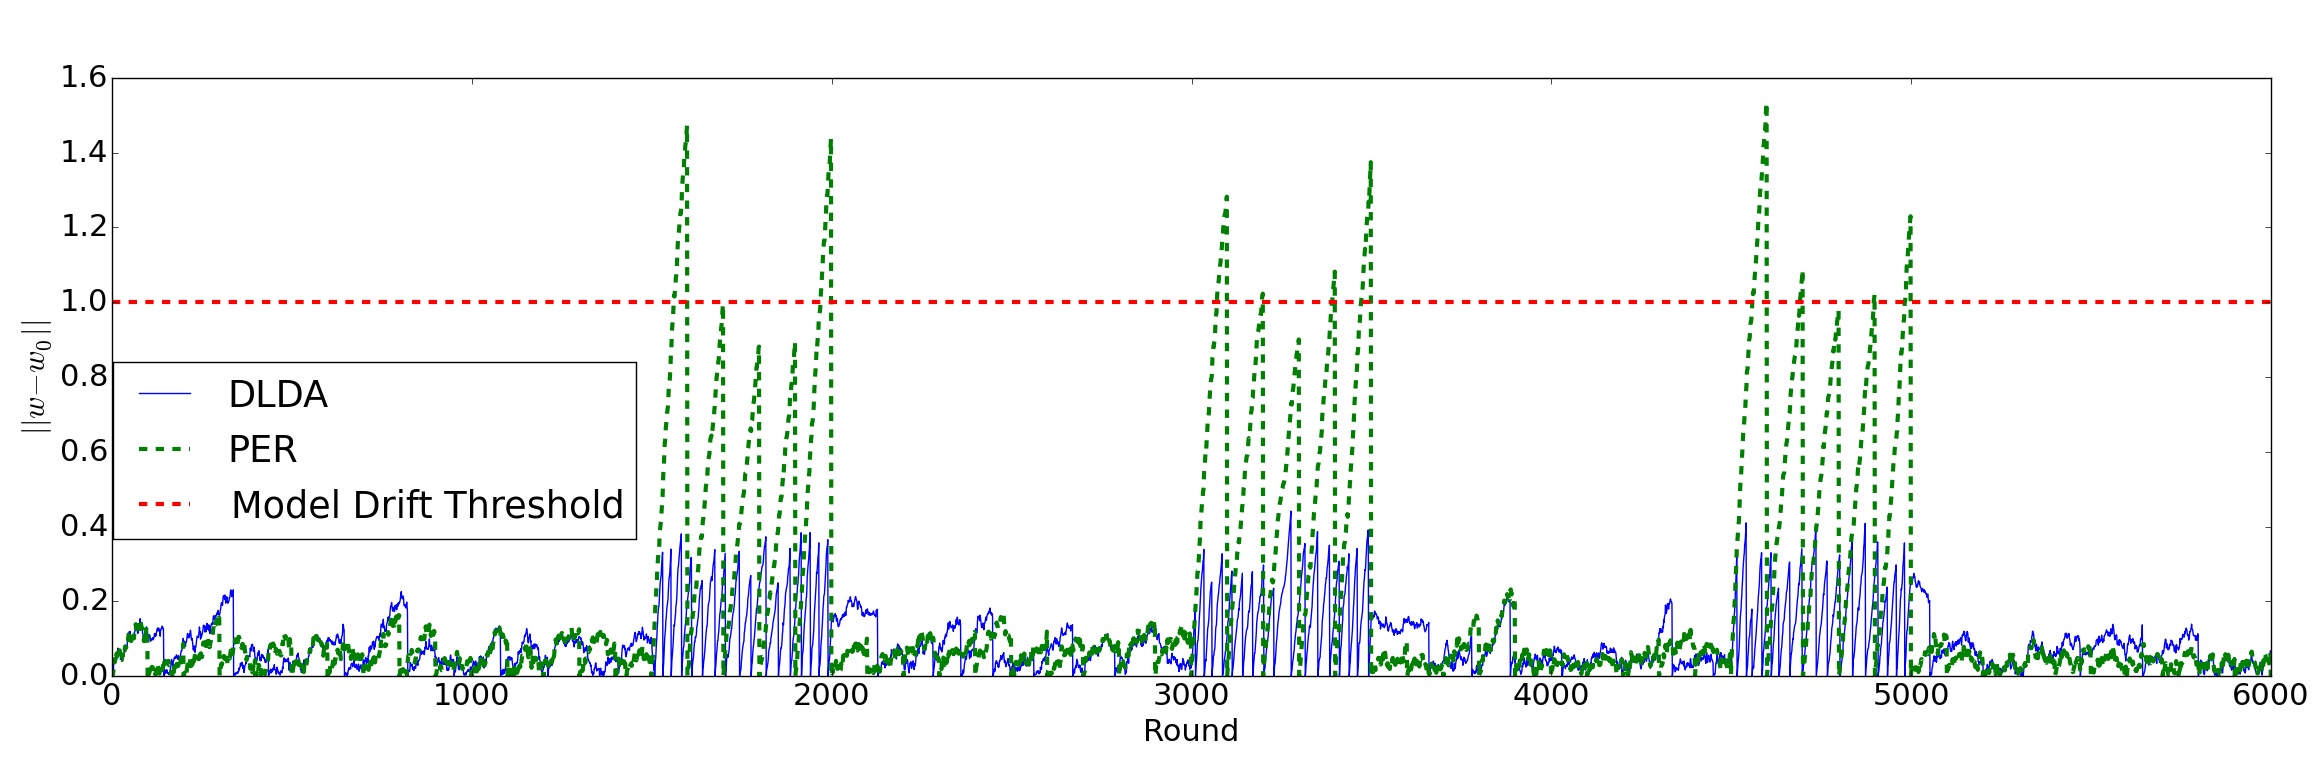
\includegraphics[width=132mm, height=50mm]{graphics/PERvsDLDAoverTime.png}
  \captionof{figure}{DLDA error (blue) vs. PER(100) error (green), for the synthetic
	data. Horizontal axis represents rounds, vertical
	axis represents the norm of the difference between the real (global) model and the current model held at the nodes. Window size is 1,000.
	The maximum allowed error (which DLDA guarantees will never be
	exceeded) is $T = 0.997$ (which corresponds to a difference of
	0.077 radians, or $4.4^{\circ}$, in the classifier's orientation). Both
	algorithms transmit the same overall number of bytes, but at different
	rounds; while PER sends alerts periodically, DLDA alerts only when the classifier may have changed. For this reason, PER suffers from a larger
	error when the two classes (and the classifier) change.}
  \label{PERvsDLDAoverTime}
\end{minipage}%
\hfill
\begin{minipage}{.26\textwidth}
  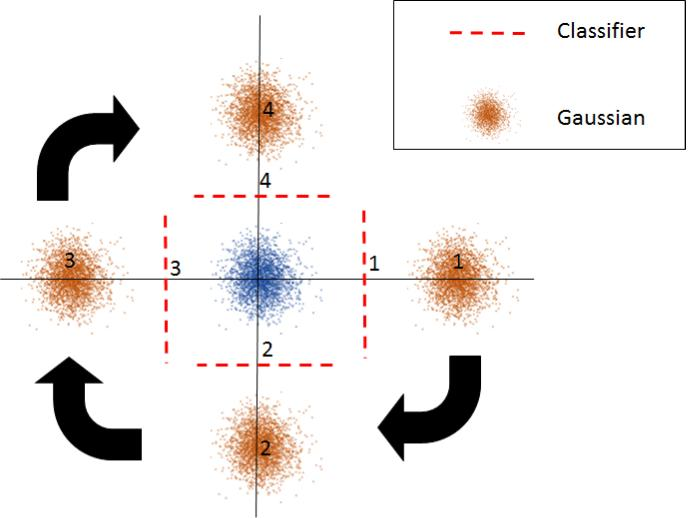
\includegraphics[width=54mm, height=45mm]{graphics/DataShiftInEarlyDetection.jpg}
  \captionof{figure}{Illustration of the generation process of the synthetic data.
	The class $P$ (denoted in blue) is fixed, while $Q$ changes three times, every 1,500 rounds (the changes are depicted by the dark arrows).}
  \label{fig:synth-data}
\end{minipage}

\end{figure*}


\label{sec:PDLDA}
DLDA triggers a synchronization whenever a single node reports a violation.
Our empirical evaluation with a large number of nodes showed that such a strict
policy results in many synchronizations even when the global model is still 
valid. This is due to the following reason: 
recall that the global condition
is that the average of certain vectors,
which are constructed separately as each node, must lie inside a convex set $\mathcal{C}$.
To guarantee this condition, DLDA demands that {\em each} of the local vectors lie in
$\mathcal{C}$. While correct, this is a gross "overkill", since, from
the same considerations underlying the central limit theorem,
fluctuations in the local vectors will with high probability cancel out, and even if a large
percentage of them is outside $\mathcal{C}$, the average will still be inside
$\mathcal{C}$. We provide here some intuition for the above claim: assume a one-dimensional
case, in which $\mathcal{C}$ is an interval, and the local vectors are random
variables. From the central limit theorem, it follows that, when averaging these
random variables, the result is much smaller (in absolute value) than the
average absolute value of the separate random variables. This also holds 
in higher dimensions, alas space limitation do not allow us to present and discuss the results; still, they imply that it is possible to relax the strict
condition DLDA imposes. 
We therefore suggest to change the synchronization policy, and synchronize only when a certain 
percentage of nodes report a violation.
This percentage, denoted {\em VT}, is empirically determined on the training set. Then,
when a node experiences a violation, it flips a coin (tuned to the value of {\em VT}),
to decide whether to submit an alert or not. In Section \ref{sec:real}, we report
results of both DLDA and PDLDA; the reduction in communication when using
PDLDA is more noticeable as the number of nodes $k$ increases.
%
%
%
\section{Evaluation}
%
We evaluated the performance of the proposed monitoring algorithms, DLDA and PDLDA, on synthetic and real data. For each dataset we simulated a distributed data stream by partitioning the data between the nodes and streaming it one sample in a round. 

\subsection{Synthetic Data Experiments}
We used synthetic data, in which we control the data generation process, to
demonstrate the communication efficiency of our method (Section \ref{sec:com_eff})
and its ability to alert when the current model isn't valid \emph{before} 
misclassifications occur (Section \ref{sec:earlydetection}). We then (Section \ref{sec:paramanal}) analyze the communication efficiency of our method as a function of
some of the data parameters.
%
%
\subsubsection{Communication Efficiency}\label{sec:com_eff}
We compare DLDA to the $P$-periodic algorithm, denoted
PER($P$), a sampling algorithm that sends updates
every $P$ rounds.
Our main performance metric is communication, measured in \textit{normalized messages} (the average number of messages sent per round by each node). 
PER can achieve arbitrarily low communication at the cost of larger model drift. However,
periodic synchronization can miss the point of change in the data; 
hence PER cannot guarantee to maintain the model error under a fixed threshold, in contrast to DLDA.  Further,
DLDA has additional advantages over PER: 
\begin{enumerate}
\item DLDA can be instantly calibrated to fit a given drift threshold, while for PER the 
interval between synchronizations can only be determined empirically. 
\item The rate at which the data evolves might change. 
While DLDA adapts to the new change rate, PER suffers from its fixed period length
which will become inappropriate for the new rate of change.
\item For a sudden change in the data, DLDA adapts\\
immediately -- the algorithm's
\textit{latency} is 0 -- while for PER the latency might be as high as the period length.
\end{enumerate}
%
In the following experiment we used a simple data generation process. There are 
10 nodes, each of which contains two data classes: $P$, a Gaussian centered
at the origin and with unit covariance matrix; and $Q$, a Gaussian also
with unit covariance matrix, but whose mean changes every 1,500 rounds, starting 
at $(1,0)$, and then changing to $(0,-1), (-1,0), (0,1)$ (see 
Figure \ref{fig:synth-data}).



%
Figure \ref{PERvsDLDAoverTime} depicts DLDA's behavior for the synthetic dataset, with 
three points in time at which the data abruptly changes. 
DLDA achieves a communication overhead of 0.01 messages per node per round, with the model 
error guaranteed to always be below the given threshold.
On the other hand,  PER(100) (whose overall communication is equal to DLDA's) doesn't maintain the
model error below the threshold (red dashed line).
Figure \ref{PERvsDLDAoverTime} shows that PER(100) does not always 
synchronize when the model drift exceeds a given threshold. 
Moreover, it triggers redundant synchronizations when there is no change in the data.
%

%

%
\subsubsection{Early Drift Detection}
\label{sec:earlydetection}
%
%
To further expound on the advantage of the proposed DLDA algorithm, we consider 
a toy example (Figure \ref{EarlyDetection}), 
in which 2D data arrives from two classes ($P$'s samples are shown as plus signs 
and $Q$'s samples as minus signs). The means of the classes change 
according to the depicted grey arrows, from time $t_I$ to $t_L$. The dark
line at an angle of $-45^{\circ}$ represents the optimal projection
direction at time $t_1$. As the classes change, this initial projection
direction remains "correct", in the sense that it still separates the
two classes; alas, at time $t_L$, the two classes have switched their
positions relative to the projection's direction, and the classifier
fails. Hence, a monitoring algorithm which only checks for misclassification
at the nodes will fail to detect the drift in the classes until it is too
late -- i.e., classification errors occur -- while DLDA will alert earlier, 
when the real (global) classifier will have changed by more than the
provided threshold (in this case 0.52 radians, or $30^{\circ}$); this point
is marked by an arrow in Figure \ref{EarlyDetection}.
%
%
\begin{figure}
	\centering
	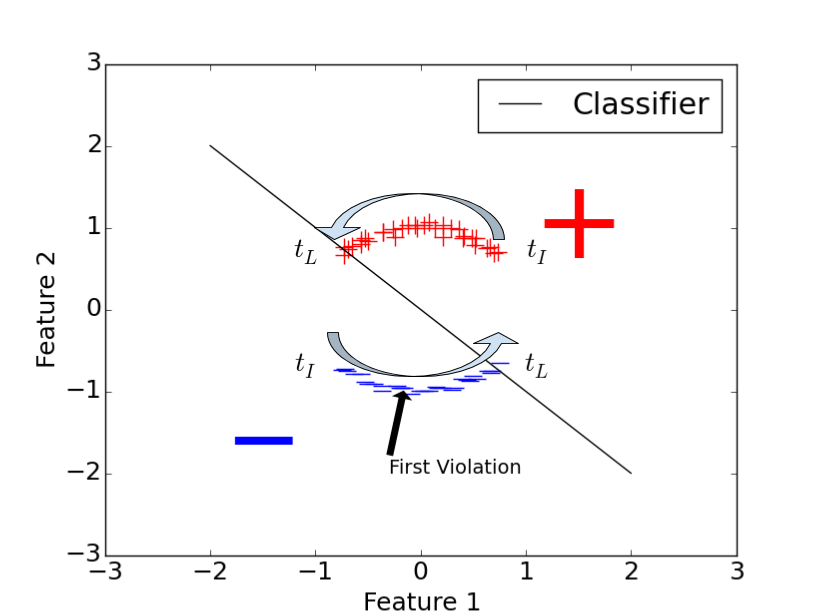
\includegraphics[width=7cm, height=40mm]{graphics/EarlyDetection.png}
	\caption{A toy example demonstrating early detection of a change in the data.
	\label{EarlyDetection}}
\end{figure}
%
%
\subsubsection{Parameter Analysis}\label{sec:paramanal}
Next, we analyze the performance of DLDA as a function of some data parameters.
~~\\
\noindent\textbf{Model Drift Threshold}  is provided by the user, and bounds
the allowed model drift (i.e. an alert should be submitted when it is crossed).
It can be defined in two ways: as the maximal angle between 
$w$ and $w_0$, or as the Euclidean distance between them. 
Figure \ref{PERvsDLDAoverError} depicts the communication overhead of DLDA 
as a function of the model drift threshold, and the minimal communication required to match 
DLDA using PER.	The data and its dynamicity are as in Section \ref{sec:com_eff}.
It can been seen that  DLDA outperforms PER for
any given model drift threshold. Importantly, note that this comparison is
heavily biased in favor of PER, since the communication overhead for
PER is measured here when it is run in hindsight; the period $P$ is determined so as to
prevent violations, but only \textit{after} the data is known. In real-life
scenarios, this is of course impossible, and not only will PER require 
more communication than DLDA, it will also miss model violations.
%
\begin{figure}
        \centering
        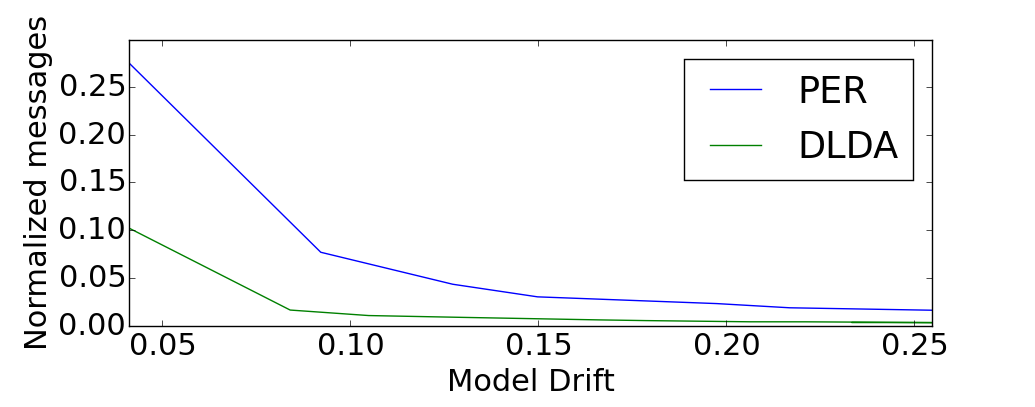
\includegraphics[width=85mm]{graphics/onlyDrift.png}
        \caption{Communication as a function of allowed model drift for DLDA and PER, the
        periodic algorithm (which is tuned to achieve the same maximal model drift as DLDA).}
        \label{PERvsDLDAoverError}
\end{figure}
%

\noindent\textbf{Node Scalability:}
Node Scalability measures how DLDA performs with different numbers of nodes.
Figure \ref{Nodes} shows the communication volume as a function of the number of nodes $k$.
We note that communication increases rather gradually, reaching 0.25\% on the fixed
data and 0.6\% on the dynamic data distributed across 25 nodes. By "fixed" data we
refer to two Gaussians as in Section \ref{sec:com_eff} whose centers do not change,
but some communication is required due to the randomness in generating
samples from the two class distributions. 

\noindent\textbf{Window Size:}
Figure \ref{WindowSize} shows how communication decreases as a result
of increasing the window size $W$.  One can increase the window size to compensate 
for other factors, such as the magnitude of 
noise present (which is quantified in our context by the standard deviation of the
data generating distribution).


\begin{figure*}
\centering
\begin{minipage}{.29\textwidth}
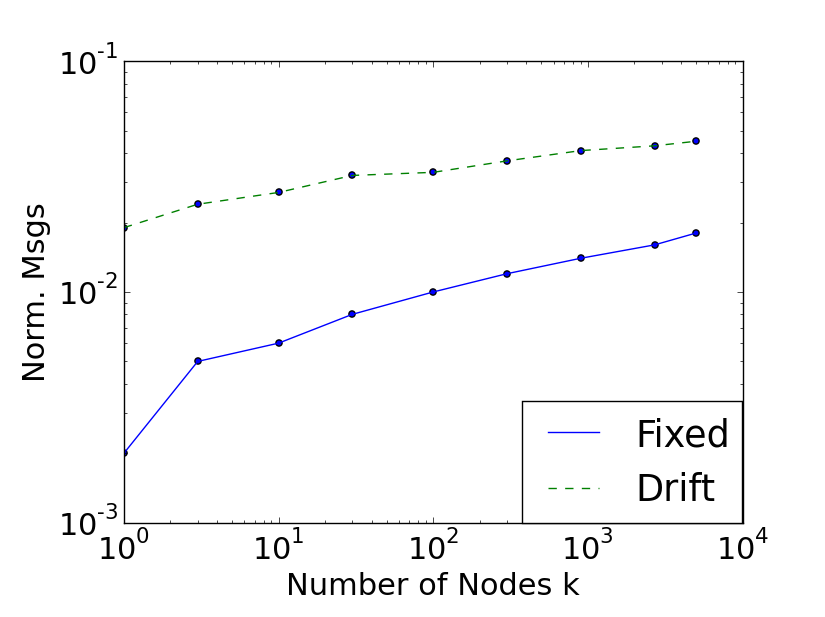
\includegraphics[width=55mm]{graphics/Nodes.png}
  \captionof{figure}{Communication as a function of the number of nodes for fixed (blue)
  and changing (dashed green line) datasets}
  \label{Nodes}
\end{minipage}%
\hfill
\begin{minipage}{.29\textwidth}
  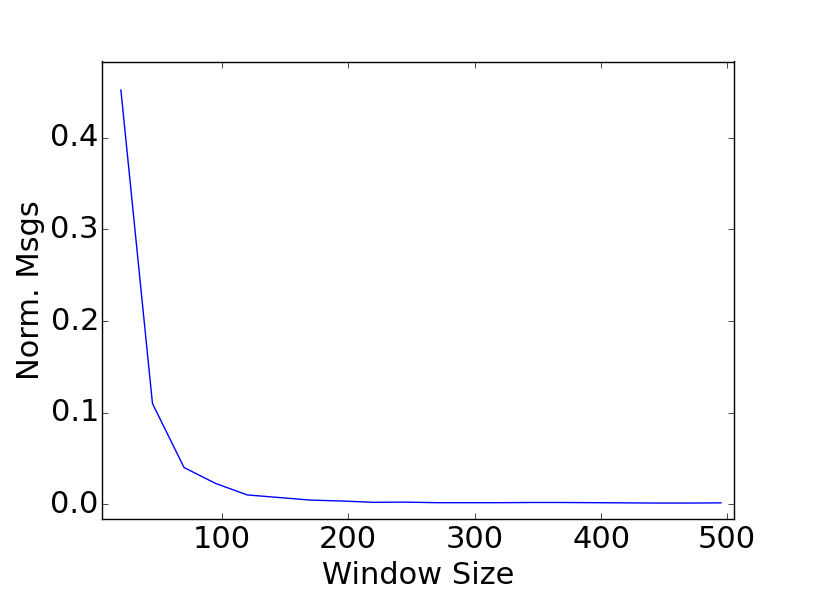
\includegraphics[width=55mm]{graphics/WindowSize.png}
  \captionof{figure}{Communication as function of window size}
  \label{WindowSize}
\end{minipage}
\hfill
\begin{minipage}{.35\textwidth}
  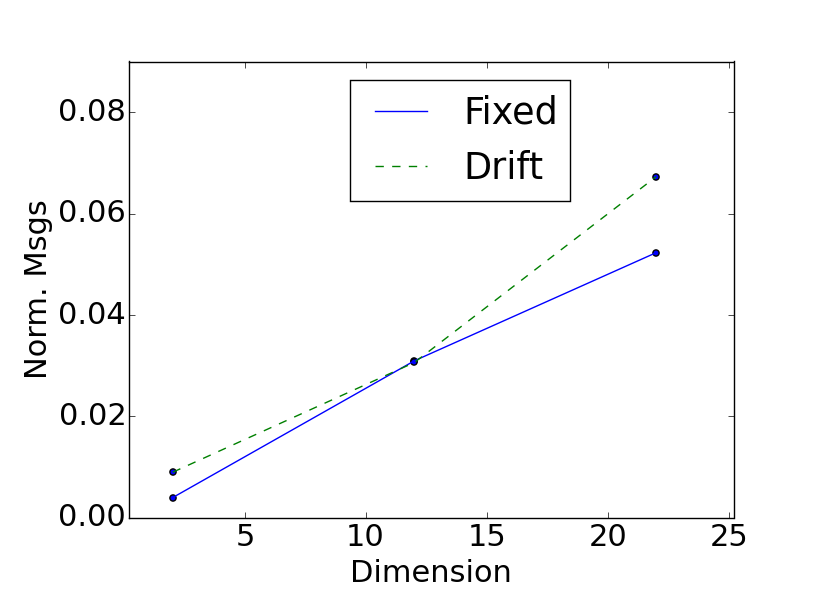
\includegraphics[width=55mm]{graphics/Dimension.png}
  \captionof{figure}{Communication as a function of input dimension for fixed (blue) and   changing (green  dashed line) datasets}
  \label{Dimension}
\end{minipage}
\end{figure*}

 %
 %
 %
Another parameter directly related to the window size is the data dimension. To simulate higher dimensions, we proceeded as for the
2D example described in detail in Section \ref{sec:com_eff} (i.e. normal distributions with a unit covariance matrix, whose centers move a distance of $\sqrt{2}$ every
1,500 rounds).
The number of 
samples required for accurate estimation of the covariance matrix increases with the dimension. In our 
settings, the number of training samples is correlated with the window size. When the window size is fixed, 
communication increases linearly with the data dimension (see Figure \ref{Dimension}).
  
%
%

\subsection{Real Data Experiments}
\label{sec:real}
We tested the algorithms on three real data sets. The first
(USENET) is too small to test the probabilistic approach (PDLDA); thus we applied
only DLDA on it.
The second (Power Consumption Monitoring) is medium size  
(distributed over 36 nodes) and we tested both DLDA and PDLDA on it.
The third (Gas Sensor Time Series Monitoring) is larger (distributed over
100 nodes). The DLDA synchronization policy is too strict for such a large number of nodes
(see Sections \ref{sec:PDLDA}),
hence on this set we tested only the probabilistic version, PDLDA.
%
\subsubsection{Message Preference Monitoring --- Usenet}
The USENET dataset \cite{usenet} is a text dataset that simulates a stream of messages 
from three newsgroups (medicine, space, baseball); 
the messages are presented sequentially to a user, who then labels them as "interesting" or "boring", 
according to his/hers personal interest; these form the two categories.
The attribute values are binary, indicating the presence or absence of 128 keywords. 
The change in the data corresponds to a change in the user's interest (e.g. from "space" to "baseball"). 

Figure \ref{usenet} shows the results of the DLDA algorithm with $W=450$. The first 450 rounds over the data correspond to
the initialization phase and are omitted. During the next 50 rounds the DLDA model drift 
(the value is calculated using the LHS in the inequality in Eq. \ref{eq:convexBound}) 
increases due to noise in the data; there is no change in the user's
interests.
From round 500 to 600 the DLDA model drift is small, and again, due only to the noise. In round 600 there is an abrupt concept
change.
From this point both the DLDA model drift and the true model drift increase until the synchronization 
in round 698, at which the error drops to zero. 
\begin{figure}[H]
	\centering
	\includegraphics[width=8cm, height=40mm]{graphics/DriftDetected.png}
	%\includegraphics[width=\textwidth]{Usenet/DriftDetected.png}
	\caption{Comparison between DLDA model drift (blue)
	and the true global model drift (green dashed), on the Usenet data set, for $k=2$, $W=450$. It can be seen that DLDA responds to the change in the data that occurs after 600 rounds (red dotted vertical line), resulting in a synchronization in 
	round 698 (blue dashed vertical line).}
	\label{usenet}
	\end{figure}
	

%
%
\subsubsection{Power Consumption Monitoring}


The Power Consumption dataset  \cite{powerSupply} contains the hourly power supply of an
Italian electric company as recorded from two sources: power supplied
by the main grid and power transformed from other grids.
The stream contains three-year power supply records
from 1995 to 1998, and our learning task is to predict whether the hour 
in question is in the day time or the night time.
The dynamicity in this stream is mainly caused by such factors as season, weather, time of day, and the differences between working days and weekends.




As discussed in Section \ref{sub:problem}, we monitor the Euclidean distance between
$w_0$ and $w$, as opposed to 1 - (cosine similarity between $w_0$ and $w$); in 
Figure \ref{CosineVsEuclideanPowerSupply}, we demonstrate that these two
measures are highly correlated.
\begin{figure}[H]
	\centering
	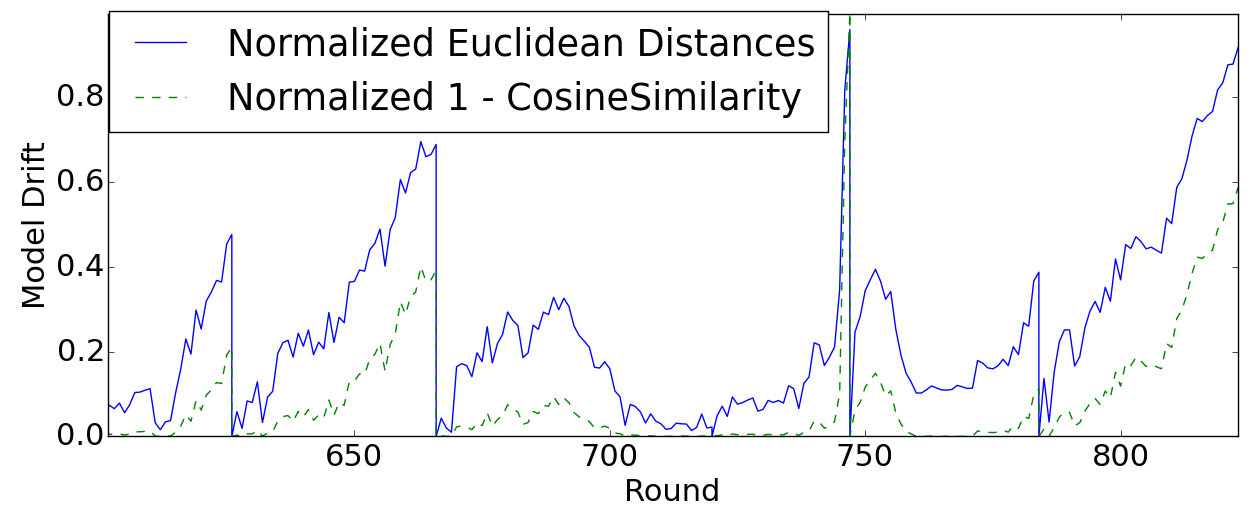
\includegraphics[width=8cm]{graphics/CosineVsEuclideanPowerSupply.png}
	%\includegraphics[width=\textwidth]{Usenet/DriftDetected.png}
	\caption{Comparison of two metrics for measuring model drift --- Euclidean distance (blue) and cosine similarity (green) --- on the power supply dataset. It can be seen that the two metrics are highly correlated.}
	\label{CosineVsEuclideanPowerSupply}
	\end{figure}


In Figure \ref{PERvsDLDAonPowerSupply}, 
DLDA is compared to PER, where the latter is tuned so that its
communication overhead will be the same as DLDA's. Note that
PER suffers from very large errors.

\begin{figure}
	\centering
	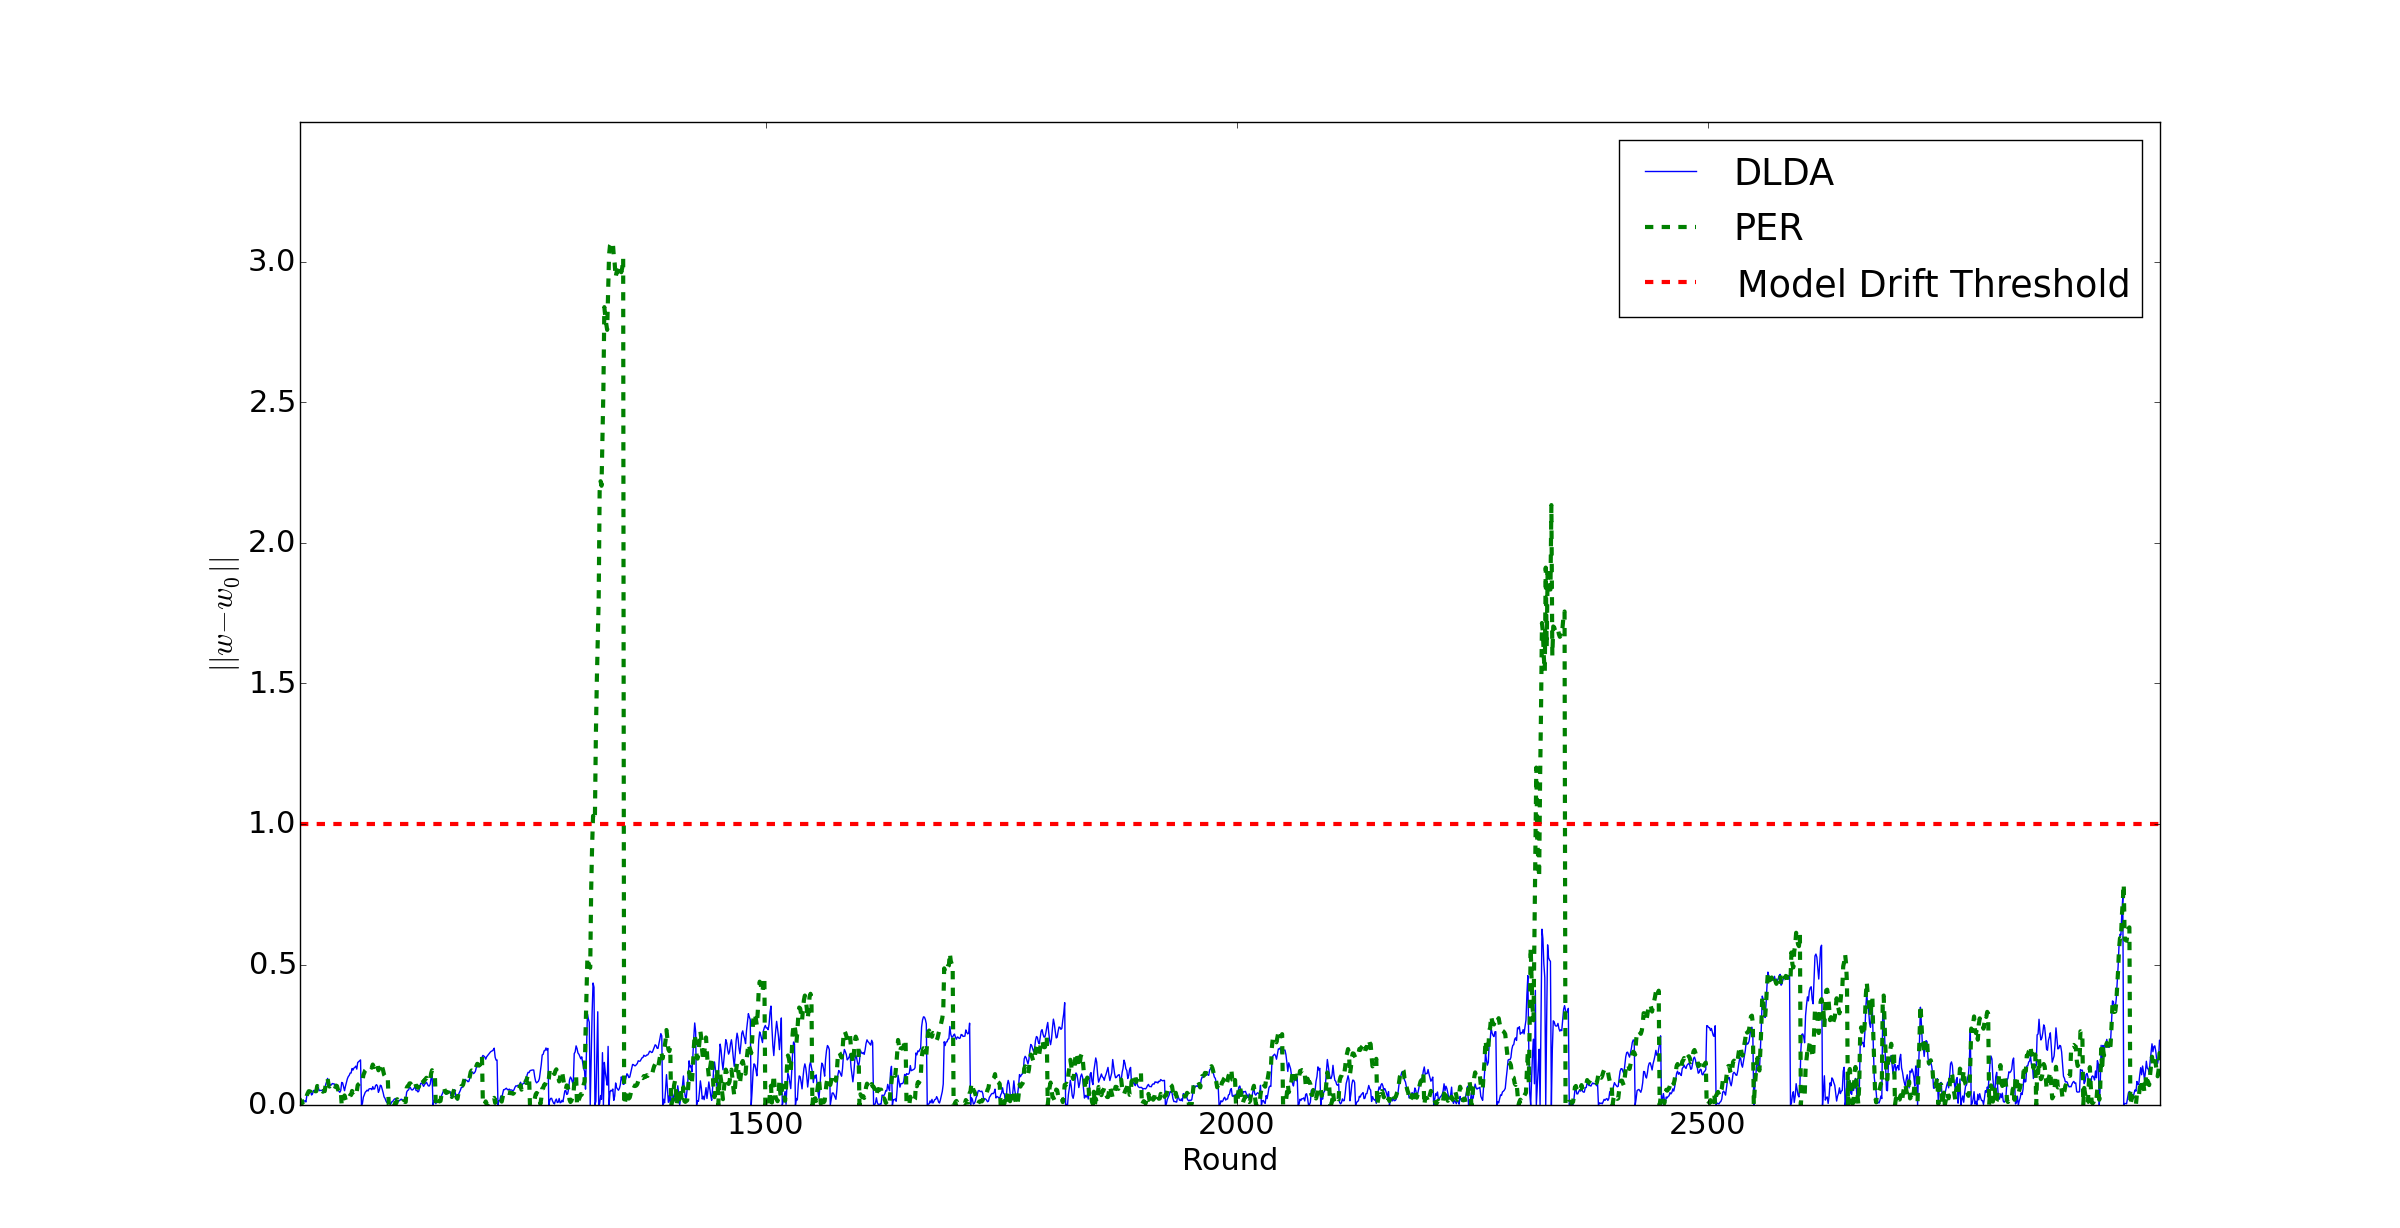
\includegraphics[width=9cm,height=40mm]{graphics/PERvsDLDAonPowerSupply.png}
	%\includegraphics[width=\textwidth]{Usenet/DriftDetected.png}
	\caption{DLDA error (blue) vs. PER(50) error (green), for the power supply
	data described above. Horizontal axis represents rounds, vertical
	axis represents the norm of the difference between the real (global) model and the 
	current model held at the nodes. Window size is 1,000.
	The maximum allowed error (which DLDA guarantees will never be
	exceeded) is $T = 0.7$ (which corresponds to a difference of
	0.8 radians, or $45^{\circ}$, in the classifier's orientation). Both
	algorithms transmit the same overall number of bytes, but at different
	rounds; while PER sends alerts periodically, DLDA alerts only when the classifier may have changed. For this reason, PER suffers from a larger
	error when the two classes change.}
	\label{PERvsDLDAonPowerSupply}
	\end{figure}


Next, we compare DLDA to the probabilistic version, PDLDA. 
Figure \ref{PowerSupplyFigures} depicts the results of the DLDA
and PDLDA algorithms. For a small number of nodes, $k=4$, and for large
window size, $W=5000$, DLDA requires only 0.003 normalized messages.
For a distributed system with more nodes ($k=36$), and a smaller window
size, $W=600$, DLDA requires 0.09 normalized messages. For PDLDA with
$k=36$ and $W=600$ and a violation threshold (VT) of 50\%, PDLDA
requires 0.02 normalized messages, much better than DLDA in the same setting;
this demonstrates a general trend -- the improvement factor of PDLDA
over DLDA is more noticeable when more nodes are present.


\begin{figure}
    \centering
    \begin{subfigure}[b]{0.5\textwidth}
        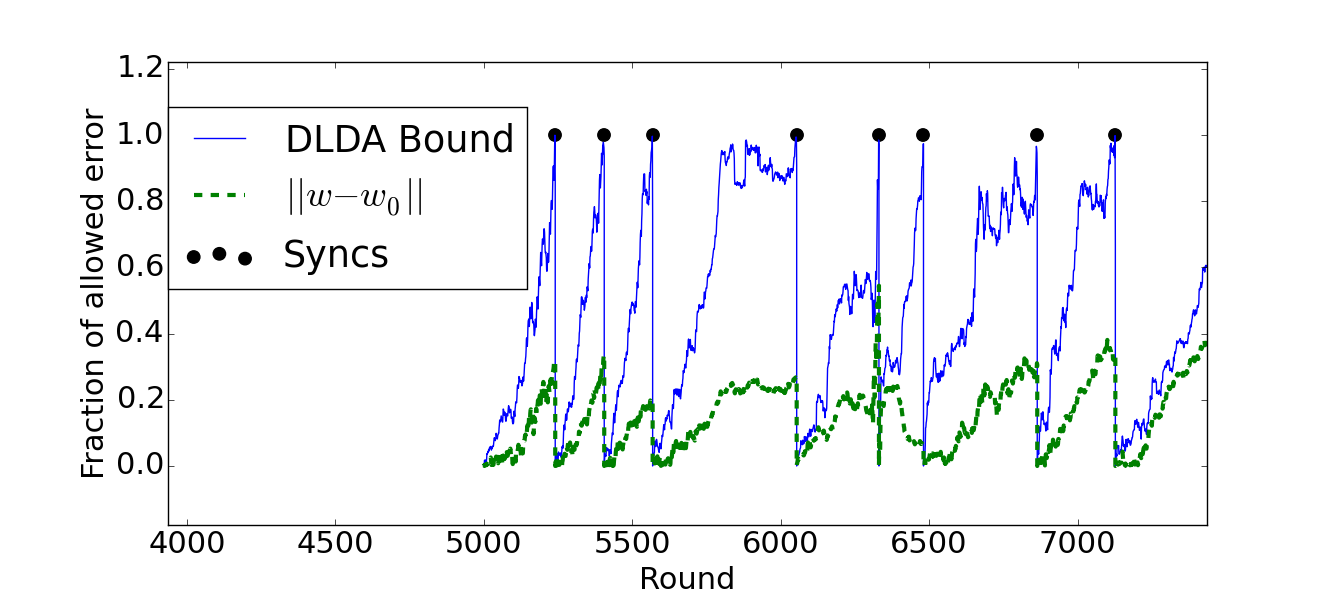
\includegraphics[width=\textwidth]{graphics/4nodes.png}
        \caption{k=4, W=5000, VT=0}
    \end{subfigure}

    \begin{subfigure}[b]{0.5\textwidth}
        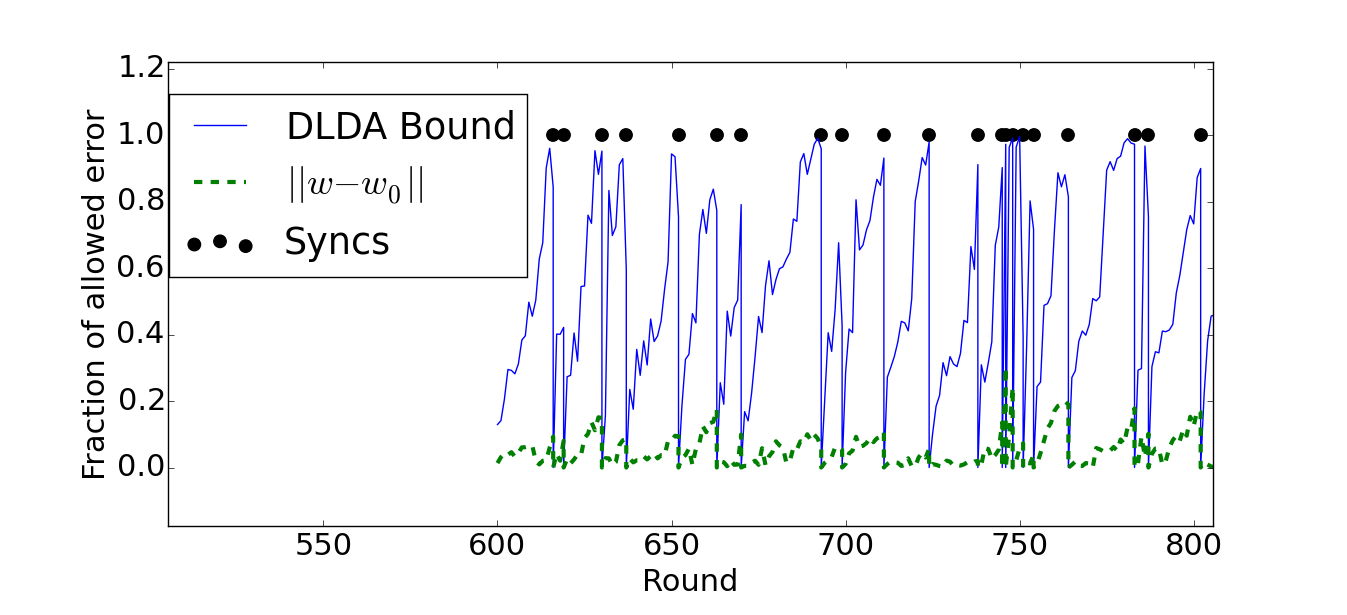
\includegraphics[width=\textwidth]{graphics/36nodes.png}
        \caption{k=36 Nodes, W=600, VT=0}
    \end{subfigure}

    \begin{subfigure}[b]{0.5\textwidth}
        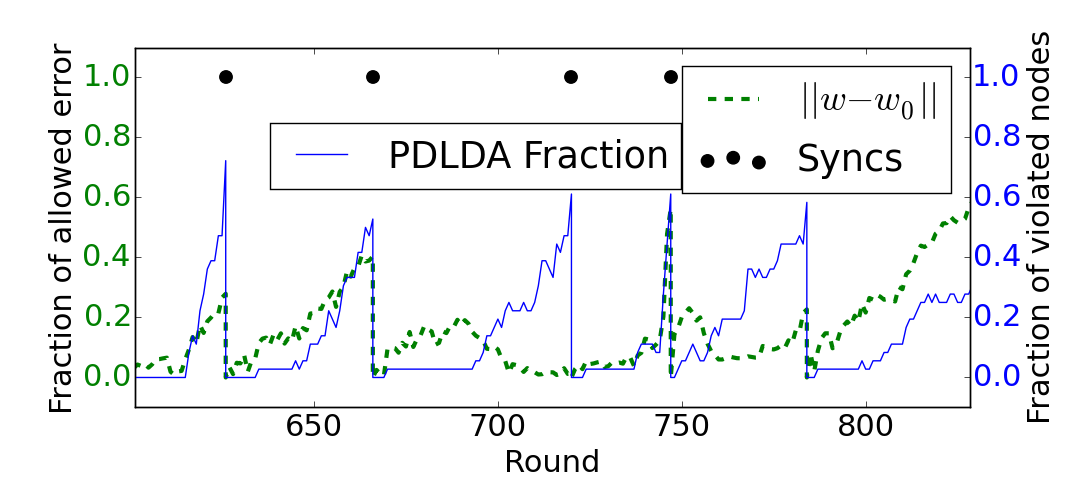
\includegraphics[width=\textwidth]{graphics/36nodesProb.png}
        \caption{k=36 Nodes, W=600, VT=18}
    \end{subfigure}
    \caption{Top and center figures depict DLDA's performance on the Power Supply data set for a small (top) and large (center) number of nodes. The blue line in (a) and (b) represents the value of the local bound, corresponding to the node with the maximum value. The green dashed line depicts the model drift (normalized by the threshold); the model is computed after the data was aggregated from all nodes. The bottom plot shows the results of PDLDA on the same dataset. The blue line in the bottom plot represents the fraction of violated nodes.}\label{PowerSupplyFigures}
    %\label{powerSupply}
\end{figure}
	
\subsubsection{Gas Sensor Time Series Monitoring} 
%
Data in this dataset \cite{fonollosa2015reservoir} consists of measurements collected
by an array of 16 chemical sensors in a lab, recording at a sampling
rate of 100Hz for 24 hours, resulting in 8378504 data points for each sensor.
During the first 12 hours the task is to detect the presence of carbon monoxide
(CO) in a mixture of chemicals, and from the 13th hour onwards the task is to detect the presence of methane, 
which corresponds to an abrupt change in the data.
Figure \ref{BigGasOverTime} demonstrates the results of the PDLDA algorithm.
First, we observe that the fraction of violated nodes (shown in blue) correlates with the true model drift (shown in green). Second, we observe two patterns of behavior, which are separated by an abrupt change in the data  (marked by the vertical red line). Before the change,  synchronization occurs every 150 rounds, and after it, 
the synchronization rate decreases to every 50 rounds. There is a transition period of about 1000 rounds that follows the point in time at which the data changes. In this interval, the sliding window is a "mixture" of the old (pre-change) data and new (post-change) data; however, once the window aggregates enough data, the algorithm stabilizes and the communication overhead drops. This experiment shows that the PDLDA algorithm detects the abrupt change in the data and adapts to the new conditions after a short period of time.
Lastly, we compare PDLDA to PER for the gas sensor data (Figure \ref{BigGasOverTime}).

\begin{figure*}[t]
\centering

\subfloat{%
  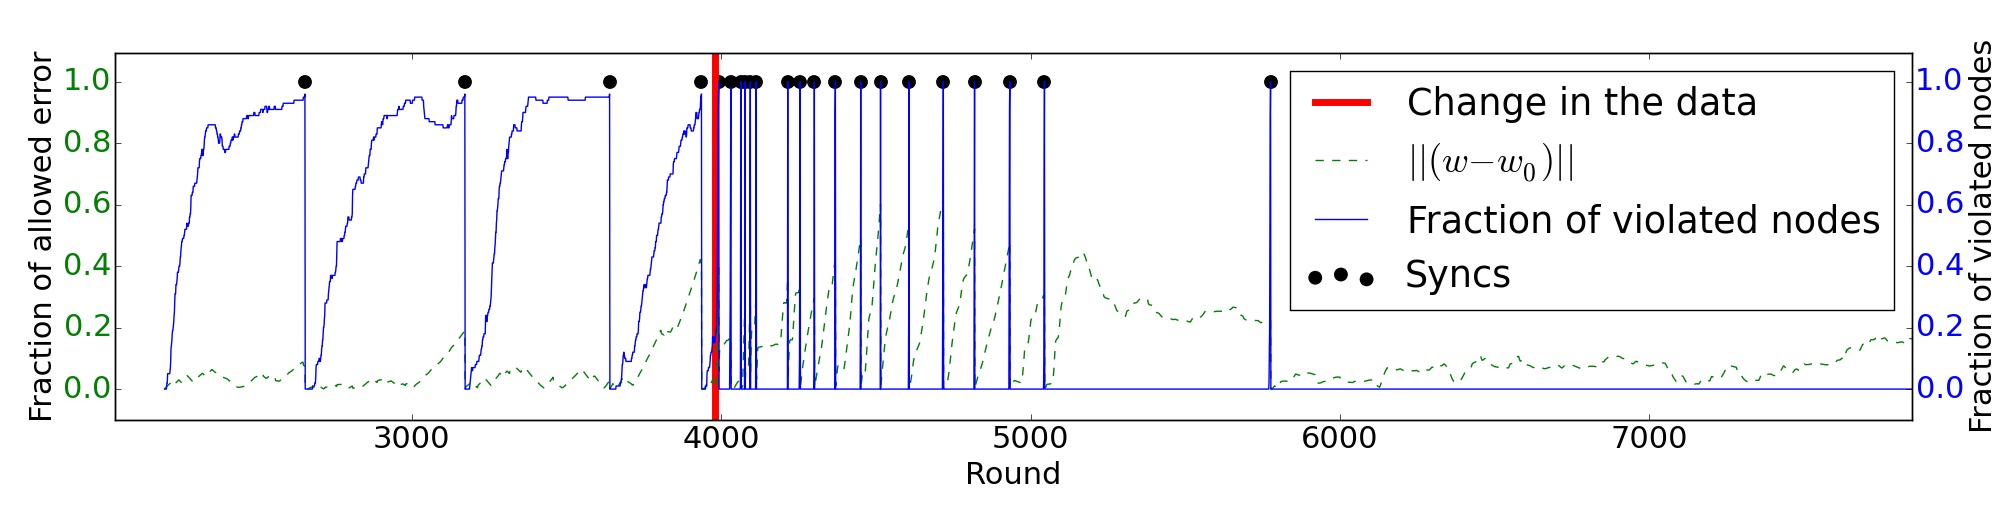
\includegraphics[width=120mm, height=37mm]{graphics/overTime100k.png}%
  \label{BigGasOverTime}%
}\qquad
\subfloat{%
  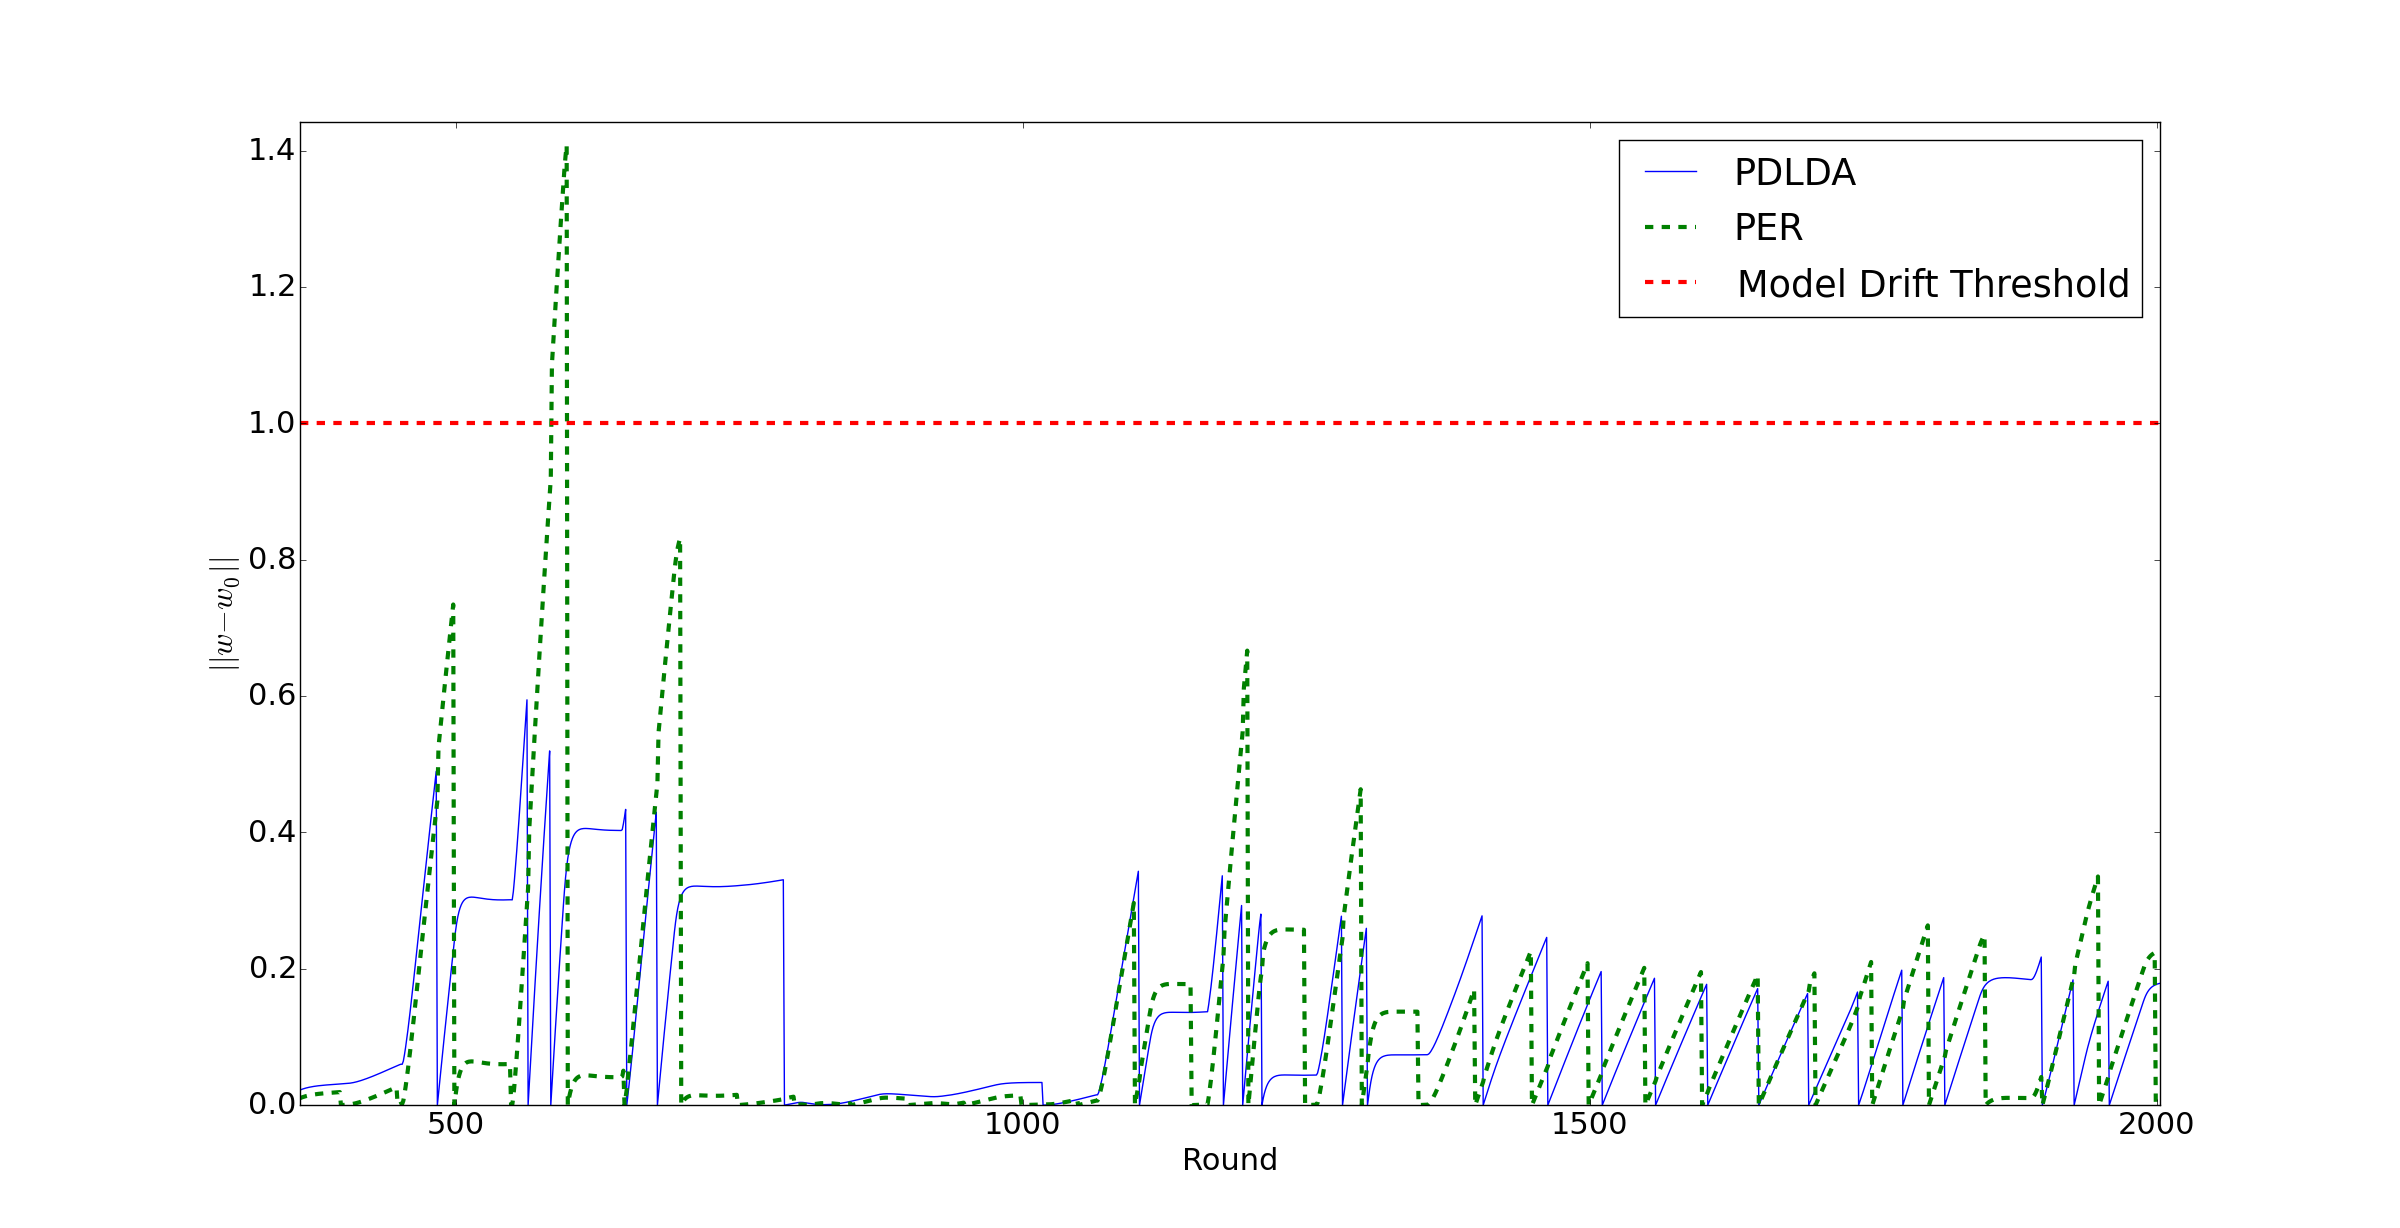
\includegraphics[width=50mm, height=36mm ]{graphics/PDLADvsPERGas.png}%
  \label{PDLADvsPERGas}%
}

\caption{In the left subfigure there is a Demonstration of PDLDA on the Gas Sensor dataset.
A comparison between the true model drift (green) to the fraction of the nodes that
are violated in the current round (blue).
There are $k=100$ nodes, and the violation threshold is
$VT=80$. While there are (naturally) more synchronizations when the data
changes abruptly (near round 4000), communication overhead drops when the
system stabilizes.
\\ In the right subfigure we show  PDLDA error (blue) vs. PER(50) error (green), for the Gas Sensor dataset. Horizontal axis represents rounds, vertical
	axis represents the norm of the difference between the real (global) model and the current model held at the nodes. Window size is 25,000.
	The maximum allowed error (which DLDA guarantees will never be
	exceeded) is $T = 0.97$ (which corresponds to a difference of
	0.24 radians, or $14^{\circ}$, in the classifier's orientation). Both
	algorithms transmit the same overall number of bytes, but at different
	rounds; while PER sends alerts periodically, DLDA alerts only when the 
	classifier may have changed. For this reason, PER results in a larger
	error when the two classes change. }
\label{BigGasOverTime}%
\end{figure*}





\section*{Conclusions}
We introduced what is, to the best of our knowledge, the first communication-efficient monitoring algorithm for a classifier in a distributed streaming environment. 
Further, we monitor the
model itself, allowing to detect model drift before misclassifications occur.
As long as all nodes meet their local condition, as defined in
the paper, the
global model is guaranteed to be valid. 

%
We evaluated both DLDA, the foolproof scheme which is guaranteed to send an
alert if the model drift is larger than a pre-defined threshold, and its probabilistic 
version PDLDA, on three real data sets.
For a small number of nodes we used DLDA, and for larger numbers of nodes 
PDLDA was tested. We showed that the proposed scheme outperforms the periodic update algorithm (PER): it maintains a smaller distance between
the last centrally computed model and the current true model, while maintaining 
lower communication overhead.

This work is hopefully an initial step in designing communication-efficient algorithms
with theoretical guarantees for monitoring classification models over dynamic, distributed data streams. One of the future directions is to extend the proposed framework to
ensembles of linear classifiers, support vector machines, and neural networks.

% BibTeX users please use one of
\bibliographystyle{abbrv}
\bibliography{bib}   % name your BibTeX data base
\nocite{*}





\end{document}
